\documentclass[journal,12pt,twocolumn]{IEEEtran}

\usepackage{graphicx}
\usepackage{setspace}
\usepackage{gensymb}
\singlespacing
\usepackage[cmex10]{amsmath}
\usepackage{amssymb}
\usepackage{xurl}
\usepackage{tabularx}
\usepackage{amsthm}
\usepackage{comment}
\usepackage{mathrsfs}
\usepackage{txfonts}
\usepackage{stfloats}
\usepackage{bm}
\usepackage{cite}
\usepackage{cases}
\usepackage{subfig}
\usepackage{arydshln}
\usepackage{longtable}
\usepackage{multirow}

\usepackage{enumitem}
\usepackage{mathtools}
\usepackage{steinmetz}
\usepackage{tikz}
\usepackage{circuitikz}
\usepackage{verbatim}
\usepackage{tfrupee}
\usepackage[breaklinks=true]{hyperref}
\usepackage{graphicx}
\usepackage{tkz-euclide}
\usetikzlibrary{automata, positioning}
\usetikzlibrary{calc,math}
\usepackage{listings}
    \usepackage{color}                                            %%
    \usepackage{array}                                            %%
    \usepackage{longtable}                                        %%
    \usepackage{calc}                                             %%
    \usepackage{multirow}                                         %%
    \usepackage{hhline}                                           %%
    \usepackage{ifthen}                                           %%
    \usepackage{lscape}     
\usepackage{multicol}
\usepackage{chngcntr}
\usepackage{blkarray}

\DeclareMathOperator*{\Res}{Res}

\renewcommand\thesection{\arabic{section}}
\renewcommand\thesubsection{\thesection.\arabic{subsection}}
\renewcommand\thesubsubsection{\thesubsection.\arabic{subsubsection}}

\renewcommand\thesectiondis{\arabic{section}}
\renewcommand\thesubsectiondis{\thesectiondis.\arabic{subsection}}
\renewcommand\thesubsubsectiondis{\thesubsectiondis.\arabic{subsubsection}}


\hyphenation{op-tical net-works semi-conduc-tor}
\def\inputGnumericTable{}                                 %%

\lstset{
%language=C,
frame=single, 
breaklines=true,
columns=fullflexible
}
\begin{document}


\newtheorem{theorem}{Theorem}[section]
\newtheorem{problem}{Problem}
\newtheorem{proposition}{Proposition}[section]
\newtheorem{lemma}{Lemma}[section]
\newtheorem{corollary}[theorem]{Corollary}
\newtheorem{example}{Example}[section]
\newtheorem{definition}[problem]{Definition}

\newcommand{\BEQA}{\begin{eqnarray}}
\newcommand{\EEQA}{\end{eqnarray}}
\newcommand{\define}{\stackrel{\triangle}{=}}
\bibliographystyle{IEEEtran}
\raggedbottom
\setlength{\parindent}{0pt}
\providecommand{\mbf}{\mathbf}
\providecommand{\pr}[1]{\ensuremath{\Pr\left(#1\right)}}
\providecommand{\qfunc}[1]{\ensuremath{Q\left(#1\right)}}
\providecommand{\sbrak}[1]{\ensuremath{{}\left[#1\right]}}
\providecommand{\lsbrak}[1]{\ensuremath{{}\left[#1\right.}}
\providecommand{\rsbrak}[1]{\ensuremath{{}\left.#1\right]}}
\providecommand{\brak}[1]{\ensuremath{\left(#1\right)}}
\providecommand{\lbrak}[1]{\ensuremath{\left(#1\right.}}
\providecommand{\rbrak}[1]{\ensuremath{\left.#1\right)}}
\providecommand{\cbrak}[1]{\ensuremath{\left\{#1\right\}}}
\providecommand{\lcbrak}[1]{\ensuremath{\left\{#1\right.}}
\providecommand{\rcbrak}[1]{\ensuremath{\left.#1\right\}}}
\theoremstyle{remark}
\newtheorem{rem}{Remark}
\newcommand{\sgn}{\mathop{\mathrm{sgn}}}
\providecommand{\abs}[1]{\vert#1\vert}
\providecommand{\res}[1]{\Res\displaylimits_{#1}} 
\providecommand{\norm}[1]{\big\lVert#1\big\rVert}
%\providecommand{\norm}[1]{\lVert#1\rVert}
\providecommand{\mtx}[1]{\mathbf{#1}}
\providecommand{\mean}[1]{E[ #1 ]}
\providecommand{\fourier}{\overset{\mathcal{F}}{ \rightleftharpoons}}
%\providecommand{\hilbert}{\overset{\mathcal{H}}{ \rightleftharpoons}}
\providecommand{\system}{\overset{\mathcal{H}}{ \longleftrightarrow}}
	%\newcommand{\solution}[2]{\textbf{Solution:}{#1}}
\newcommand{\solution}{\noindent \textbf{Solution: }}
\newcommand{\cosec}{\,\text{cosec}\,}
\providecommand{\dec}[2]{\ensuremath{\overset{#1}{\underset{#2}{\gtrless}}}}
\newcommand{\myvec}[1]{\ensuremath{\begin{pmatrix}#1\end{pmatrix}}}
\newcommand{\mydet}[1]{\ensuremath{\begin{vmatrix}#1\end{vmatrix}}}
\newcommand*{\permcomb}[4][0mu]{{{}^{#3}\mkern#1#2_{#4}}}
\newcommand*{\perm}[1][-3mu]{\permcomb[#1]{P}}
\newcommand*{\comb}[1][-1mu]{\permcomb[#1]{C}}
\numberwithin{equation}{subsection}
\makeatletter
\@addtoreset{figure}{problem}
\makeatother
\let\StandardTheFigure\thefigure
\let\vec\mathbf
\renewcommand{\thefigure}{\theproblem}
\def\putbox#1#2#3{\makebox[0in][l]{\makebox[#1][l]{}\raisebox{\baselineskip}[0in][0in]{\raisebox{#2}[0in][0in]{#3}}}}
     \def\rightbox#1{\makebox[0in][r]{#1}}
     \def\centbox#1{\makebox[0in]{#1}}
     \def\topbox#1{\raisebox{-\baselineskip}[0in][0in]{#1}}
     \def\midbox#1{\raisebox{-0.5\baselineskip}[0in][0in]{#1}}
\vspace{3cm}
\title{\textbf{LINEAR SYSTEMS AND SIGNAL PROCESSING \\ ASSIGNMENT 5}}
\author{GANJI VARSHITHA - AI20BTECH11009}
\maketitle
\newpage
\bigskip
\renewcommand{\thefigure}{\arabic{figure}}
\renewcommand{\thetable}{\arabic{table}}
Download latex codes from 
%
\begin{lstlisting}
https://github.com/VARSHITHAGANJI/EE3900_VECTORS_ASSIGNMENTS/blob/main/QUADRATIC_FORMS_ASSIGNMENT5/QUADRATIC_FORMS_ASSIGNMENT5.tex
\end{lstlisting}



Download all python codes from
\begin{lstlisting}
https://github.com/VARSHITHAGANJI/EE3900_VECTORS_ASSIGNMENTS/blob/main/QUADRATIC_FORMS_ASSIGNMENT5/plot_code.py
\end{lstlisting}




\section*{QUESTION}
\textbf{Quadratic Forms 2.6}


Find the area lying in the first quadrant and bounded by the circle $ \Vec{x}\Vec{x}^\top = 4 $ and the lines x = 0 and x = 2.
 

\section*{SOLUTION}
The general equation of a circle is 
\begin{align}
\label{eq:1}
\Vec{x}\Vec{x}^\top - 2 \Vec{O}^\top \Vec{x} + \norm{O}^{2}-r^2=0
\end{align}
Given equation of the circle is
\begin{align}
\label{eq:2}
\Vec{x}\Vec{x}^\top = 4
\end{align}
Comparing \eqref{eq:2} with \eqref{eq:1}, we get
\begin{align}
\label{eq:3}
\Vec{O}=\myvec{0 \\ 0}\\
\label{eq:4}
r=2
\end{align}
Given lines are
\begin{align}
\label{eq:5}
L_{1}: \: \myvec{1 & 0}\Vec{x}=0 \\
\label{eq:6}
L_{2}: \: \myvec{1 & 0}\Vec{x}=2
\end{align}
The angle made by lines $L_{1}$ and $L_{2}$ with the x axis i.e $\myvec{0 & 1}\Vec{x}=0$ is
\begin{align}
\label{eq:7}
\cos \theta = {}&\frac{\myvec{1 \\ 0}^\top \myvec{0 & 1}}{\norm{\myvec{1 & 0}}\norm{\myvec{0 & 1}}}\\
\label{eq:8}
={}& 0\\
\label{eq:9}
\implies \theta = 90^{\circ}
\end{align}
The area of sector thus obtained is
\begin{align}
\label{eq;10}
\frac{\theta^{\circ}}{360^{\circ}}\pi r^2 ={}&\frac{90^{\circ}}{360^{\circ}}\pi r^2\\
\label{eq:11}
={}&\frac{\pi}{4}2^2\\
\label{eq:12}
={}&\pi
\end{align}
\begin{figure}[h]
\centering
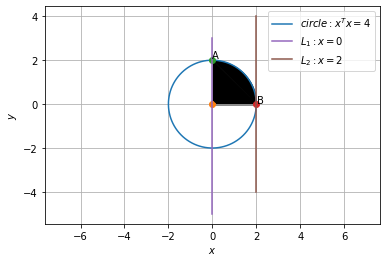
\includegraphics[width=\columnwidth]{q5}
\caption{Plotting the region bounded by circle and lines in first quadrant}

\end{figure}
		
\end{document}
